\documentclass[12pt]{ctexart}
\usepackage{xeCJK}
\usepackage{fontspec}
\usepackage{titlesec}
% 设置全局字体为楷体
\setCJKmainfont{KaiTi}[
    BoldFont={SimHei}, % 使用黑体作为粗体
    ItalicFont={STXinwei}, % 使用楷体作为斜体
    BoldItalicFont={SimHei} % 使用黑体作为粗斜体
]
% 设置英文字体
\setmainfont{Times New Roman}

% 设置section标题的字号
\titleformat{\section}
  {\normalfont\fontsize{26}{31.2}\bfseries}
  {}
  {0pt}
  {}

% 设置页面
\usepackage{amsmath}
\usepackage{hyperref}
\hypersetup{breaklinks=true}
\usepackage{geometry}
\usepackage{tabularx}
\usepackage{array}
\usepackage{float}
\usepackage{wrapfig}
\usepackage{lastpage}
\usepackage{titlesec}
\usepackage{indentfirst}
\usepackage{tikz}
\usepackage{everypage}
\usepackage{caption}
\captionsetup[figure]{labelformat=empty}
\usepackage{xcolor}
\usepackage{listings}
\PassOptionsToPackage{hyphens}{url}
\usepackage{url}
\usepackage{xurl}
\usepackage{hyperref}
\hypersetup{breaklinks=true}
\usepackage{tikz}
% 插图片
\usepackage{graphicx}
% 设置摘要页缩减 
\usepackage{changepage}
% 设置页眉页脚
\usepackage{fancyhdr}
\setlength{\headheight}{12.64723pt}
\addtolength{\topmargin}{-0.64723pt}
% 清空页眉页脚
\pagestyle{fancy}
% 设置列表缩进
\usepackage[shortlabels]{enumitem}
% 设置修改默认的section标题大小
\usepackage{titlesec}
\titleformat*{\section}{\LARGE}
\titleformat*{\subsection}{\Large}
\titleformat*{\subsubsection}{\Large}
% 使用数学宏包
\usepackage{amsmath}
% 设置表格的列格式
\usepackage{array}
% 三线表宏包
\usepackage{booktabs}
% 设置产考文献不输出默认名
\usepackage{etoolbox}
\patchcmd{\thebibliography}{\section*{\refname}}{}{}{}
% 设置等宽的代码字体
\setmonofont{Courier New}
% 颜色
\usepackage{xcolor}

\lstset{
  language=Matlab,
  basicstyle=\small\ttfamily,       % 稍小的等宽字体
  keywordstyle=\color{blue}\bfseries,  % 关键字蓝色加粗
  commentstyle=\color{gray}\itshape,   % 注释灰色斜体
  stringstyle=\color{orange},         % 字符串橙色
  numbers=left,                       % 左侧显示行号
  numberstyle=\tiny\color{gray},     % 行号样式
  stepnumber=1,                       % 每行都编号
  numbersep=8pt,                      % 行号与代码间距
  showstringspaces=false,             % 不用特殊符号显示空格
  breaklines=true,                    % 自动断行
}

% 绘制页面边框
\usepackage{everypage}
\AddEverypageHook{
  \begin{tikzpicture}[remember picture, overlay]
    \draw[thick] ([xshift=0.5cm, yshift=0.5cm]current page.south west) rectangle ([xshift=-0.5cm, yshift=-0.5cm]current page.north east);
  \end{tikzpicture}
}

% 设置自定义字体
\newfontfamily\customfont{Freestyle Script}
\newfontfamily\haettenfont{Haettenschweiler}
\setCJKmainfont{Microsoft YaHei}
\setmainfont{TeX Gyre Termes}
\renewcommand{\contentsname}{Table of Contents}

% 引用格式
\newenvironment{mdquote}
{%
  \par\noindent
  \begin{list}{}{%
      \setlength{\leftmargin}{1em}%
      \setlength{\rightmargin}{0pt}%
      \setlength{\itemindent}{0pt}%
      \setlength{\listparindent}{\parindent}%
      \setlength{\topsep}{0.5\baselineskip}%
  }
  \item[\textbf{>}\ ]\itshape
}
{\end{list}\par}


\begin{document}

% 标题页
\begin{titlepage}
    \centering
    \vspace*{96pt}
    \fontsize{26}{31.2}\selectfont{Introdution to Compressed Sensing}\par % 主标题
    \vspace{39pt}
    \fontsize{22}{26.4}\selectfont{\haettenfont v1 .0\normalfont}\par % 版本
    \vspace{52.8pt}
    \fontsize{18}{21.6}\selectfont{Author: \customfont{Lancet Ross}}\par % 作者
    \fontsize{18}{21.6}\selectfont{Last Edited on: Jul 30th, 2025}\par % 最后编辑时间
    \vfill
\end{titlepage}

% 目录页
\newpage
\thispagestyle{empty}
\small
\tableofcontents
\newpage
% 目录页后面是第一页
\setcounter{page}{1}

% 开始写正文
% 设置正文的页边距
\newgeometry{top=3cm, left=3.5cm, right=3.5cm}
% 设置正文的页眉页脚
\fancyhf{}
\fancyhead[C]{ }
% 此处修改右上角页码
\fancyhead[R]{Page \thepage\ of\ \NoHyper\pageref{LastPage}\endNoHyper}
\fancyhead[L]{\customfont Introdution to Compressed Sensing}
\fancyfoot[C]{\bfseries\thepage}

% 序言页
\newpage
\titleformat{\section}[block]{\normalfont\Large\bfseries\centering}{}{0pt}{}
\section*{\textbf{Preface}}
\addcontentsline{toc}{section}{Preface}

Human beings have run into 21st century. The rapid development of information technology
has greatly increased the amount of data we need. It's clear that the real world is analog
and the digital world is discrete so that signal sampling is the necessary way to convert
the real world into the digital one. \textbf{Shannon-Nyquist sampling theorem} tells us
that the sampling rate should be at least twice the maximum frequency of the signal to
avoid aliasing, and this frequency is called the Nyquist frequency. However,
Shannon-Nyquist sampling theorem is faced with a problem that us humans wants to decrease
the cost of data sampling and storage. Is there a way to break through the
Shannon-Nyquist sampling theorem and sample the signal at a lower rate? The answer is yes,
and this is the \textbf{Compressed Sensing}.

We often call Compressed Sensing as CS for short, and also Compressive Sampling. Its
Chinese name is \textbf{压缩感知}, translated by Professor Qionghai Dai from Tsinghua
University. Compressed Sensing is a new theory that can reconstruct the original signal
from a small number of samples, which is much less than the Nyquist rate. For example, if
we lost \textbf{70\%} of the samples, we can still reconstruct the original signal with a
high probability. This is much unbelievable for us. Therefore someone said that Compressed
Sensing is the most important discovery in information theory since Shannon-Nyquist
sampling theorem.

To learn such a powerful theory is not easy. We need to start from the signal
transformation, and then some basic concepts like sparse representation and norm. After
that we will introduce the reconstruction algorithms, which is the most important part
of Compressed Sensing. In this tutorial we will mainly introduce greedy algorithms and
iterative thresholding algorithms. The final part is the concept of Compressed Sensing
and its applications. I still strongly recommended that you should have learned Teacher
Xue's \textbf{Signals and Systems} and \textbf{Linear Algebra} (no matter the teacher is 
Professor Liu or other teachers) before you start. 

Well, I was learning CS and writing this tutorial at the same time. Just like my last Linux
tutorial, I was writing it while I was at home. To be honest, I don't know much about CS,
and I even don't know if I can write this tutorial well. But I will try my best. If you find
any mistakes or have any suggestions, please feel free to contact me.

Let's rock and roll!

\begin{flushright}
  Lancet Ross\\
  Jul 24th, 2025
\end{flushright}

\newpage
\thispagestyle{empty}
\begin{center}
    \vspace*{96pt}
    \fontsize{60}{60}\customfont{1}\par
    \fontsize{26}{31.2}\section{\textbf{Signal transformation}}\par % 标题
    \vspace{25pt}
    \fontsize{18}{21.6}\customfont{\textit{What we know is not much. What we do not know is
    immense. --- P. S. Laplace}}\par % 名言
    \vfill
\end{center}

\fontsize{12}{14}
\newpage
\subsection{\textbf{Discrete Fourier Transform}}

We have learned CTFT, CTFS, LT, DTFT and ZT in Signals and Systems. In this section
we will introduce the Discrete Fourier Transform (DFT).

\subsubsection{\textbf{Defination}}

The Discrete Fourier Transform (DFT) is created on the basis of the Discrete
Fourier Series (DFS). If we call a periodic signal $x_p(t)$, then we should notice
that it can't be two-side Z transformed, because it is not absolutely summable.
However, we can use the Discrete Fourier Series to represent it:
\[
  X_p(k) = \sum_{n=0}^{N-1} x_p(n)\,e^{-j\frac{2\pi}{N}kn},\quad k=0,1,\dots,N-1.
\]

And the inverse:
\[
  x_p(n) = \frac{1}{N}\sum_{k=0}^{N-1} X_p(k)\,e^{j\frac{2\pi}{N}kn},\quad n=0,1,
  \dots,N-1.
\]

For convience, we define that:
\[
  W = e^{-j\frac{2\pi}{N}}.
\]

Then we can rewrite the DFT and IDFT:
\[
  X(k) = \sum_{n=0}^{N-1} x(n)\,W^{kn},\quad k=0,1,\dots,N-1.
\]

\[
  x(n) = \frac{1}{N}\sum_{k=0}^{N-1} X(k)\,W^{-kn},\quad n=0,1,\dots,N-1.
\]

\subsubsection{\textbf{Properties}}

DFT processes discrete periodic signals. Its core is to periodic extend a finite
discrete sequence and still get a finite discrete sequence after DFT.

\paragraph{\textbf{Linearity}}\mbox{}\\
\[
  DFT[a_1x_1(n) + a_2x_2(n)] = a_1DFT[x_1(n)] + a_2DFT[x_2(n)].
\]

\paragraph{\textbf{Shifting}}\mbox{}\\

\textit{Firstly we need to notice 2 things:}

\textit{1. $x_p(n) = x((n))_N$ This means that $x_p(n)$ is a periodic signal with 
period $N$}

\textit{2. $x(n) = x_p(n)R_N(n) \quad R_N(n) = u(n) - u(n-N)$}

\textbf{Time shifting} is that if $y(n) = x((n-m))_NR_N(n)$ (This is called Circular
Shift m samples), then we have$Y(k) = W^{mk}X(k)$

\textbf{Frequency shifting} is that if $Y(k) = X((k-l))_NR_N(k)$, then we have
$y(n) = W^{-nl}x(n)$

\paragraph{\textbf{Circular Convolution}}\mbox{}\\

In \textbf{time} domain if $y(n) = x(n)h(n)$ then we have:
\[
 Y(k) = \frac{1}{N}\sum_{n=0}^{N-1} X(l)H((k-l))_NR_N(k) = \frac{1}{N}\sum_{n=0}^{N-1}
H(l)X((k-l))_NR_N(k).
\]

In \textbf{frequency} domain if $Y(k) = X(k)H(k)$ then we have:
\[
  y(n) = \sum_{n=0}^{N-1} x(m)h((n-m))_NR_N(n) = \sum_{n=0}^{N-1} h(m)x((n-m))_NR_N(n).
\]

\paragraph{\textbf{Parseval's Theorem}}\mbox{}\\
\[
  \sum_{n=0}^{N-1} |x(n)|^2 = \frac{1}{N}\sum_{k=0}^{N-1} |X(k)|^2.
\]

\paragraph{\textbf{DFT and ZT}}\mbox{}\\
\[
  X(k) = X(z)|_{z=W^k}
\]

\[
  X(z)|_{z=e^{-j\frac{2\pi}{N}k}} = X(k)
\]

\subsubsection{\textbf{Fast Fourier Transform}}

The Fast Fourier Transform (FFT) is an algorithm to compute the DFT efficiently. The DFT
has a time complexity of $O(N^2)$, which is not efficient for large $N$. The FFT reduces
the time complexity to $O(N\log N)$ by exploiting the symmetries in the DFT.

Computers use FFT to compute the DFT, You can use fft() function in MATLAB, Python and
so on.

Here's an example of using FFT in MATLAB:
\begin{lstlisting}[language=Matlab]
%% FFT_example
clear; clc; close all;

%% parameters
Fs = 1000;            % sampling frequency
T = 1/Fs;             % sampling period
L = 1500;             % length of signal
t = (0:L-1)*T;        % time vector

S = 0.7 * sin(2*pi*50*t) + sin(2*pi*120*t);
X = S + 2*randn(size(t));

%% time domain
figure('Name','FFT','NumberTitle','off')
subplot(2,1,1)
plot(t,X,'b','LineWidth',1.2)
title('time domain')
xlabel('time')
ylabel('amplitude')
grid on
xlim([0 0.2])

%% FFT
Y = fft(X);
P2 = abs(Y/L);
P1 = P2(1:L/2+1);
P1(2:end-1) = 2*P1(2:end-1);

% frequency axis
f = Fs*(0:(L/2))/L;

%% frequency domain
subplot(2,1,2)
plot(f,P1,'r','LineWidth',1.5)
title('frequency domain')
xlabel('frequency')
ylabel('amplitude')
grid on
xlim([0 250])

\end{lstlisting}

\begin{figure}[H]
  \centering
  \includegraphics[width=0.9\textwidth]{assets/1.1 Discrete Fourier Transform/FFT
  Example.png}
  \caption{MATLAB FFT Example}
\end{figure}

\subsection{\textbf{Non Uniform Fourier Transform}}

\subsubsection{\textbf{Defination}}

FFT is fast, but also limited. The fact puts us into a dilemma: DFT requires that the
sampling points are uniformly distributed, but in real world the sampling points are not
always like this. So we have to find a way to deal with this problem. In this section we
will introduce the Non Uniform Fourier Transform (NUFT).

Let's take an example:

\begin{lstlisting}[language=Matlab]
t = sort([0:0.1:9.9, rand(1,20)*100]);
f = sin(2*pi*0.5*t) + 0.5*cos(2*pi*2*t);
\end{lstlisting}

This signal has 100 uniformly distributed sampling points and 100 non-uniformly ones,
How to solve this problem by NUFT?

\subsubsection{\textbf{Process}}

In fact, NUFT puts the non-uniformly distributed sampling points into uniformly
distributed ones, and then uses FFT. Academically speaking, NUFT uses convolution and
interpolation to reflect those sampling points into uniform grids. For example, above
200 sampling points can be distributed into (0,20) by every 0.1 seconds (according to
the size of interval and oversampling factor actually). Then use NUFFT.

\paragraph{\textbf{Kernel}}\mbox{}\\

To interpolate sampling points, we introduce Kernel. Kernel is a function that
describes the shape of the interpolation.

\textbf{Gaussian Kernel} is a common kernel function, which is defined as:
\[
  \phi(x) = e^{-\frac{x^2}{2\sigma^2}}.
\]

$x$ is the distance from the sampling point to the grid point, and $σ$ is a width
parameter. Gaussian Kernel is simple that its accuracy and complexity grow with $σ$.

\textbf{Kaiser-Bessel Kernel (KB Kernel)} is another common kernel function, which is
defined as:
\[
  \phi(x) =
  \begin{cases}
    \dfrac{I_0\!\bigl(\beta\sqrt{1 - (2x/\omega)^2}\bigr)}{I_0(\beta)}, & |x|\le
    \tfrac{w}{2},\\ 0, & \text{otherwise},
  \end{cases}
\]

Here $I_0$ is the zero-order modified Bessel function, $\omega$ is the kernel’s support
width (typically 6–12), $\beta$ is the shape parameter given by
\[
  \beta = \pi\sqrt{\frac{w^2}{\alpha^2} - 0.5},
\]
and $\alpha$ is the oversampling factor (commonly 1.25, 1.5 or 2.0). The KB Kernel is
theoretically optimal and used in libraries such as FINUFFT, though its computation is
more involved.

\paragraph{\textbf{gridding}}\mbox{}\\

The size of the grid equals to the oversampling factor times the original signal's size.
The steps of gridding are as follows: seek grid range, calculate the weight of kernel,
weighted accumulate to grid points, oversample the grid points.

\subsubsection{\textbf{FINUFFT}}

Things we talked above are the basic concepts of NUFT. There are many libraries
that can help us to do NUFT. For example the most famous one, \textbf{FINUFFT}.

FINUFFT is divided into 3 parts: finufft1d1, finufft1d2 and finufft1d3. They are
used to solve signals which are non-uniform in time domain, frequency domain and
both.

Here's a comparison of FINUFFT and FFT for a continuous signal:
\begin{lstlisting}[language=Matlab]
%% FINUFFT_example
clear; clc; close all;

%% parameters
fs = 1000;              % sampling frequency
L = 1500;               % length of signal
t_uniform = (0:L-1)/fs; % time vector

%% calculation
% normalize time to [-pi, pi]
T_total = max(t_uniform) - min(t_uniform);
t_norm = (t_uniform - min(t_uniform)) / T_total * 2*pi - pi;

% create signal
x = 0.7*sin(2*pi*60*t_uniform) + sin(2*pi*120*t_uniform);

% finufft1d1
ms = floor(L/2)+1;
Y = finufft1d1(t_norm, x, -1, 1e-6, ms);

% frequency domain
tmp = abs(Y/L);
X = tmp(1:floor(L/2)+1);
X(2:end-1) = 2*X(2:end-1);

% frequency axis
f_target = (0:ms-1) * fs / L - fs/4;

%% FFT
Y_fft = fft(x, L);
P2 = abs(Y_fft/L);
P1 = P2(1:floor(L/2)+1);
P1(2:end-1) = 2*P1(2:end-1);
f_fft = (0:floor(L/2)) * fs / L;

%% create figure
figure('Position', [100, 100, 1200, 600]);

% FINUFFT
subplot(1,2,1);
stem(f_target, X, 'LineWidth', 1.2, 'Marker', 'none');
title('FINUFFT');
xlabel('frequency');
ylabel('|X(f)|');
xlim([0, 200]);
grid on;
set(gca, 'FontSize', 12);

% FFT
subplot(1,2,2);
stem(f_fft, P1, 'LineWidth', 1.2, 'Marker', 'none', 'Color', [0.8 0.2 0.2]);
title('FFT');
xlabel('frequency');
ylabel('|X(f)|');
xlim([0, 200]);
grid on;
set(gca, 'FontSize', 12);

%% add title
sgtitle('FINUFFT vs FFT', 'FontSize', 16, 'FontWeight', 'bold');
\end{lstlisting}

\begin{figure}[H]
  \centering
  \includegraphics[width=0.95\textwidth]{assets/1.2 Non Uniform Fourier Transform/FINUFFT
  vs FFT.png}
  \caption{FINUFFT vs FFT}
\end{figure}

\subsection{\textbf{Discrete Cosine Transform}}

\subsubsection{\textbf{Introduction}}

Do you think such a question: Nature doesn't have many complex signals, most of the signals
are real. So why we use FT and create a complex basis function $e^{-j\omega t}$? Why not
just use cosine? Well this is what \textbf{Discrete Cosine Transform (DCT)} do.

\subsubsection{\textbf{Defination}}

DCT is a twice long DFT which for real even functions. Assume we have a right-side signal
$x(m)$, which is blue in the figure below. and we fold it back to the left side, which Is
the red part:

\begin{figure}[H]
  \centering
  \includegraphics[width=0.95\textwidth]{assets/1.3 Discrete Cosine Transform/DCT
  Process 1.png}
  \caption{DCT Process 1}
\end{figure}

Now the new signal is not even, it has x=-0.5 as its symmetry axis. So we move it 0.5 to
the right, now it's even:

\begin{figure}[H]
  \centering
  \includegraphics[width=0.95\textwidth]{assets/1.3 Discrete Cosine Transform/DCT
  Process 2.png}
  \caption{DCT Process 2}
\end{figure}

Now DFT can be used to this signal:
\begin{align}
X(k) &= \sqrt{\frac{1}{2N}}\sum_{m'=-N+\tfrac12}^{N-\tfrac12} x\bigl(m'-\tfrac12\bigr)
        \cos\!\Bigl(\frac{2\pi m'n}{2N}\Bigr)\\
     &= \sqrt{\frac{2}{N}}\sum_{m'=\tfrac12}^{N-\tfrac12}x\bigl(m'-\tfrac12\bigr)
        \cos\!\Bigl(\frac{2\pi m'n}{2N}\Bigr)
        \quad(n = 0,1,\dots,N-1)
\end{align}

By replacing $m'$, we can obtain:
\[
  X(k) = \sqrt{\frac{2}{N}}\sum_{m=0}^{N-1} x(m)\cos\!\Bigl(\frac{(2m+1)n\pi}{2N}\Bigr)
  \quad(n = 0,1,\dots,N-1)
\]

However, now the DCT matrix is not orthogonal, so we need to normalize it:
\begin{align}
  X(k) &= a(n)\sum_{m=0}^{N-1} x(m)\cos\!\Bigl(\frac{(2m+1)n\pi}{2N}\Bigr)
  \quad(n = 0,1,\dots,N-1)\\
  a(n) &= \begin{cases}
    \sqrt{\frac{1}{N}}, & n = 0,\\
    \sqrt{\frac{2}{N}}, & n = 1,2,\dots,N-1.
  \end{cases}
\end{align}

This is the DCT, which is also called \textbf{DCT-II}, and IDCT is called \textbf{DCT-III}.
\begin{align}
  x(n) &= \beta(k)\sum_{k=0}^{N-1} X(k)\cos\!\Bigl(\frac{(2m+1)n\pi}{2N}\Bigr)
  \quad(m = 0,1,\dots,N-1)\\
  \beta(k) &= \begin{cases}
    \sqrt{\frac{1}{N}}, & m = 0,\\
    \sqrt{\frac{2}{N}}, & m = 1,2,\dots,N-1.
  \end{cases}
\end{align}

More than that, like FFT, DCT also has a fast algorithm called \textbf{Fast DCT (FDCT)}
with a time complexity of $O(NlogN)$. Its core is to break the DCT basis matrix into many
smaller matrices to reduce the calculation complexity.

\subsubsection{\textbf{Application}}

DCT is widely used in image and audio compression, such as \textbf{JPEG} and \textbf{MP3}.
It is especially effective for signals with a lot of low-frequency components, as it can
represent these components with fewer coefficients.


\subsection{\textbf{Short Time Fourier Transform}}

\subsubsection{\textbf{Introduction}}

Till now all we talked is in FT's field. FT is good, but not that good. It's a blind
method that can't tell us the time information of the signal. Here's an proper example:

\begin{figure}[H]
  \centering
  \includegraphics[width=0.95\textwidth]{assets/1.4 Short Time Fourier Transform/FT's
  disadvantage.png}
  \caption{FT's disadvantage}
\end{figure}

If the blue signal is F1, the red one is F2, then F2 is the reverse of F1. But their
FTs are the same. It shows that FT can only find the frequency weight but can't tell
where the weight is.

It's also simple to solve this problem. Just divide the signal into 2 parts, the previous
second and the next second, do FT on both parts, and then we can get the time information.

This is called split by window in STFT. So there is a new concept called
\textbf{window function}.

\subsubsection{\textbf{Defination}}

STFT uses a window function to divide the signal into some parts, and then do FT on
each part. The core of STFT is to change the basis function to $e^{-j\omega t}y_{window}(t)$.

There are so many window functions, the most colorful one is the gate function $g_\tau(t)$
(This is also called Gabor Transform). All window functions are compact supported, which
means that they are non-zero only in a finite interval.

\subsubsection{\textbf{Process}}

We set the window function as $g_{0.5}(t)$ and $t_s$ is the time shift of it. Here's the
result of STFT:
\begin{lstlisting}[language=Matlab]
%% STFT_example
clear; clc; close all;

%% 参数
Fs = 1000;            % sampling frequency
T = 1/Fs;             % sampling period
L = 2000;             % length of signal
t = (0:L-1)*T;        % time vector

% create signal
X1 = [sin(2*pi*20*t(1:L/2)), 2*sin(2*pi*10*t(L/2+1:end))];
X2 = [2*sin(2*pi*10*t(1:L/2)), sin(2*pi*20*t(L/2+1:end))];

%% create figure
figure('Name','STFT','NumberTitle','off', 'Position', [100, 100, 1200, 600])

% window function
window_size = 0.5;
ts = [0.5, 1.0, 1.5, 2.0]; % t_s
y_positions = [0, 0.5, 1.0, 1.5];
colors = {'b', 'g', 'r', 'm'};
freq_range = [0, 50];

%% STFT of x1
subplot(1,2,1)
hold on; grid on;
title('X1')
xlabel('frequency')
ylabel('ts')
zlabel('amplitude')
view(45, 30)

for i = 1:length(ts)
    t_end = ts(i);
    t_start = t_end - window_size;

    idx_start = find(t >= t_start, 1);
    idx_end = find(t <= t_end, 1, 'last');
    segment = X1(idx_start:idx_end);
    seg_length = length(segment);

    % FFT
    Y = fft(segment);
    P2 = abs(Y/seg_length);
    P1 = P2(1:floor(seg_length/2)+1);
    P1(2:end-1) = 2*P1(2:end-1);

    % frequency axis
    f = Fs*(0:(floor(seg_length/2)))/seg_length;

    freq_idx = find(f >= freq_range(1) & f <= freq_range(2));
    f_display = f(freq_idx);
    P1_display = P1(freq_idx);

    plot3(f_display, repmat(y_positions(i), size(f_display)), P1_display, ...
          'Color', colors{i}, 'LineWidth', 2)
end

% axis
xlim(freq_range)
ylim([-0.1 1.6])
zlim([0 2.5])
set(gca, 'FontSize', 12)
legend('0s', '0.5s', '1s', '1.5s', 'Location', 'northeast')

%% STFT of x2
subplot(1,2,2)
hold on; grid on;
title('X2')
xlabel('frequency')
ylabel('ts')
zlabel('amplitude')
view(45, 30)

for i = 1:length(ts)
    t_end = ts(i);
    t_start = t_end - window_size;

    idx_start = find(t >= t_start, 1);
    idx_end = find(t <= t_end, 1, 'last');
    segment = X2(idx_start:idx_end);
    seg_length = length(segment);

    % FFT
    Y = fft(segment);
    P2 = abs(Y/seg_length);
    P1 = P2(1:floor(seg_length/2)+1);
    P1(2:end-1) = 2*P1(2:end-1);

    % frequency axis
    f = Fs*(0:(floor(seg_length/2)))/seg_length;

    freq_idx = find(f >= freq_range(1) & f <= freq_range(2));
    f_display = f(freq_idx);
    P1_display = P1(freq_idx);

    plot3(f_display, repmat(y_positions(i), size(f_display)), P1_display, ...
          'Color', colors{i}, 'LineWidth', 2)
end

% axis
xlim(freq_range)
ylim([-0.1 1.6])
zlim([0 2.5])
set(gca, 'FontSize', 12)
legend('0s', '0.5s', '1s', '1.5s', 'Location', 'northeast')

% title
sgtitle('STFT', 'FontSize', 16, 'FontWeight', 'bold')
\end{lstlisting}

\begin{figure}[H]
  \centering
  \includegraphics[width=0.95\textwidth]{assets/1.4 Short Time Fourier Transform/STFT
  Example.png}
  \caption{STFT Example}
\end{figure}

STFT can distinguish the time information of the signal, every 0.5 seconds. When facing
more complex signals, we can use smaller window size to get more detailed time information.

\subsection{\textbf{Continuous Wavelet Transform}}

\subsubsection{\textbf{Introduction}}

Heisenberg Uncertainty Principle tells us that we can't get the time and frequency
information of a signal at the same time. The resolution of time and frequency domain
is always negative correlated. This means that if we want to get more detailed time
information, we have to sacrifice the frequency information, and vice versa.

For low frequency signals we hope to get higher frequency resolution, then the window
function will be wider. For high frequency signals we hope to get higher time
resolution, then the window function will be narrower.

It's certain that the time resolution will be lost to zero without window function. And
the window width of STFT is fixed, which means that its resolution is also fixed. This is
not good for us, because we want to get a varaible resolution. So we need a new window
function.

This is the \textbf{wavelet mother function}.

\begin{figure}[H]
  \centering
  \includegraphics[width=0.95\textwidth]{assets/1.5 Continuous Wavelet Transform/Wavelet
  mother function.png}
  \caption{Wavelet mother function}
\end{figure}

\subsubsection{\textbf{Defination}}

Wavelet mother function is not a single function, but a family of functions. There are
4 conditions for a wavelet mother function:
\begin{enumerate}
  \item It should be a compact supported function.
  \item Its integral is zero.
  \item Admissibility condition: $\int_{-\infty}^{\infty} |\hat{\phi}(\omega)|^2
  \frac{d\omega}{\omega} < \infty$. Here $\hat{\phi}(\omega)$ is the FT of $\phi(t)$.
  \item Orthogonality condition: $\int_{-\infty}^{\infty} \phi(t) \phi(t - t_0) dt = 0$
  for $t_0 \neq 0$.
\end{enumerate}

The admissibility condition and orthogonality condition ensure that the wavelet transform
can be invertible.

The wavelet mother function has no fixed frequency but a range. Therefore, Wavelet Transform
is more like a Band Pass Filter (BPF).

Here's the \textbf{wavelet funtion}:
\[
  \psi^*(\tau,s) = \frac{1}{\sqrt{s}}\psi(\frac{t}{s}-\tau)
\]

It's very easy to understand. $\tau$ is the time shift, $s$ is the scale factor. $\frac{1}
{\sqrt{s}}$ is the normalization factor, which ensures that the energy is preserved.

When $s$ is small, the wavelet function is squezzed, which means that it has a high time
resolution. When $s$ is large, the wavelet function is stretched, which means that it has
a high frequency resolution. This is exactly what we want.

And Continuous Wavelet Transform (CWT) is similar to FT, which it just changes the basis
function to $\psi^*(\tau,s)$.

\subsubsection{\textbf{Process}}

See these 2 figures$^{[1]}$. The yellow signal is the original signal, the blue one is the wavelet
function. Figure 1 chooses a small $s$ to filter the high frequency part and figure 2
chooses a large $s$ to filter the low frequency part. This is the idea of CWT.

\begin{figure}[H]
  \centering
  \includegraphics[width=0.75\textwidth]{assets/1.5 Continuous Wavelet Transform/CWT
  Example 1.png}
  \caption{From: THE WAVELET TUTORIAL, Robi Polikar}
\end{figure}
\begin{figure}[H]
  \centering
  \includegraphics[width=0.75\textwidth]{assets/1.5 Continuous Wavelet Transform/CWT
  Example 2.png}
  \caption{From: THE WAVELET TUTORIAL, Robi Polikar}
\end{figure}

Teacher Xue said, no matter what kind of signal transformation it is, the core is the
basis function. All transformations perform inner product operation between the basis
function and the signal. FT's basis function is $e^{-j\omega t}$, which has no compact
support condition. STFT's basis function is $e^{-j\omega t}y_{window}(t)$, which a fixed
window width gives a fixed resolution. CWT's basis function is $\psi^*(\tau,s)$, which has
a variable window width and a variable resolution. That's why Wavelet Transform wins.

In the end, there are many wavelet mother functions, such as Haar wavelet, Daubechies
wavelet and so on. Use what kind of wavelet mother function depends on the signal
you want to process. It is always beneficial to refer to others' materials.

\subsection{\textbf{Discrete Wavelet Transform}}

\subsubsection{\textbf{Introduction}}

CWT solves the problem of STFT. However, CWT can only process continuous signals.
Like CTFT changes to DFT, CWT also has a discrete version, which is called DWT.
This is according to computer's discreteness and finiteness.

\subsubsection{\textbf{Defination}}

Mallat created a new algorithm to process DWT, which is called \textbf{Mallat Algorithm}.
The core of Mallat Algorithm is to use a pair of low-pass filter and high-pass filter
to decompose the signal into 2 parts: low frequency part and high frequency part.

Let the original signal pass through a LPF $h[n]$ and a HPF $g[n]$, if the highest
frequency of the signal is $\pi$, then the highest part(high frequency coefficient) is
($\pi/2, \pi$) and the lowest part is ($0, \pi/2$)(low frequency coefficient). This
process is called \textbf{half sub-band filtering}.

The process of diluting the sampling points by a factor of N is called N-fold
\textbf{subsampling}, on the other hand, the process of increasing the sampling points
by a factor of N is called N-fold \textbf{upsampling} (also called interpolation).

Both half sub-band filtering and 2-fold subsampling is called \textbf{wavelet decomposition}.

After first decomposition, now keep the high frequency coefficient and decompose the
low frequency coefficient twice, three times, and so on. Until it can't be
decomposed anymore (that is to say, 1).

Subsampling makes time resolution worse, but frequency resolution better. So we get our
result, variable resolution.

Here's the process$^{[1]}$ of Mallat Algorithm:
\begin{figure}[H]
  \centering
  \includegraphics[width=1\textwidth]{assets/1.6 Discrete Wavelet Transform/Mallat
  Algorithm.png}
  \caption{From: THE WAVELET TUTORIAL, Robi Polikar}
\end{figure}

\subsubsection{\textbf{Example}}

\begin{lstlisting}[language=Matlab]
%% DWT_example
clear; clc; close all;

%% Parameters
fs = 1000;              % sampling frequency
N = 64;                 % number of samples
t = (0:N-1)/fs;         % time vector

% Original signal
f1 = 50;
f2 = 100;
x_clean = 2*sin(2*pi*f1*t) + sin(2*pi*f2*t);

% Gaussian white noise
SNR = 10;
noise_power = var(x_clean) / (10^(SNR/10));
noise = sqrt(noise_power) * randn(1, N);
x_noisy = x_clean + noise;

%% Wavelet decomposition
wavelet = 'db4';        % db4 wavelet
level = 4;              % 4 levels of decomposition

[c, l] = wavedec(x_noisy, level, wavelet);

% Reconstruct approximation and detail coefficients at each level
A = cell(1, level);
D = cell(1, level);
for k = 1:level
    A{k} = wrcoef('a', c, l, wavelet, k);  % Approximation at level k
    D{k} = wrcoef('d', c, l, wavelet, k);  % Detail at level k
end

% Reconstruction
x_recon = waverec(c, l, wavelet);

% Compute frequency bands for each sub-band
freq_bands = cell(1, level+1);
for k = 1:level
    high_freq = fs / (2^k);
    low_freq  = fs / (2^(k+1));
    freq_bands{level-k+2} = sprintf('D%d: %.1f–%.1f Hz', k, low_freq, high_freq);
end
freq_bands{1} = sprintf('A%d: 0–%.1f Hz', level, fs/(2^(level+1)));

%% create figure
figure('Position', [100, 100, 800, 900]);
numPlots = level + 2;

% 1. Noisy signal
subplot(numPlots, 1, 1);
plot(t, x_noisy, 'color', [0.6 0 0.6], 'LineWidth', 1.5);
title(sprintf('Noisy Signal (SNR=%ddB, N=%d)', SNR, N));
xlabel('time'); ylabel('amplitude');
xlim([t(1), t(end)]); grid on; ylim([-5, 5]);

% 2. Approximation factor
subplot(numPlots, 1, 2);
plot(t, A{level}, 'r', 'LineWidth', 1.5);
title(freq_bands{1});
xlabel('time'); ylabel('amplitude');
xlim([t(1), t(end)]); grid on; ylim([-3, 3]);

% 3. Detail factor
for k = level:-1:1
    subplot(numPlots, 1, level - k + 2);
    plot(t, D{k}, 'color', [0 0.5 0], 'LineWidth', 1.2);
    title(freq_bands{level - k + 2});
    xlabel('time'); ylabel('amplitude');
    xlim([t(1), t(end)]); grid on;
    % Adjust y-axis based on subband
    if k == 4 || k == 3
        ylim([-3, 3]);
    else
        ylim([-1.5, 1.5]);
    end
end

% 4. Reconstructed signal
subplot(numPlots, 1, numPlots);
plot(t, x_recon, 'b', 'LineWidth', 1.5);
hold on;
plot(t, x_noisy, 'r--', 'LineWidth', 1.2);
xlabel('time'); ylabel('amplitude');
xlim([t(1), t(end)]); grid on; ylim([-5, 5]);
legend('Reconstructed Signal', 'Noisy Signal', 'Location', 'best');
title('Reconstructed Signal');

sgtitle('DWT', 'FontSize', 12);
\end{lstlisting}

\begin{figure}[H]
  \centering
  \includegraphics[width=0.95\textwidth]{assets/1.6 Discrete Wavelet Transform/DWT
  Example.png}
  \caption{DWT Example}
\end{figure}

Approximation factor is the low frequency coefficient and detail factor is the high frequency
coefficient. Only D3 and D4 need to be retained, as the frequency components of the signal
are 50Hz and 100Hz. The error is extremely small, which shows the good performance of DWT.

\newpage
\thispagestyle{empty}
\begin{center}
    \vspace*{96pt}
    \fontsize{60}{60}\customfont{2}\par
    \fontsize{26}{31.2}\section{\textbf{Basic Concepts}}\par % 标题
    \vspace{25pt}
    \fontsize{18}{21.6}\customfont{\textit{Information is the resolution of uncertainty.
    --- Cluade Shannon}}\par % 名言
    \vfill
\end{center}

\newpage
\subsection{\textbf{Sparsity}}

\subsubsection{\textbf{Defination}}

As we all know, Compressed Sensing is a typical problem of Machine Learning. So we need
to understand what sparsity is before starting.

Think a simple question: how to tell your friend in crowd? We just need to remember some
features of him, such as his face, height, clothes and so on. In fact the most common way
is to remember his face, because it's the most distinctive feature. There are so many
features on one's face, but we only need to remember a few of them. This is called
\textbf{sparsity}. Sparsity is a concept that describes the situation where only a few
elements in a vector are non-zero or significant, while the rest are zero or almost zero.

Except this, we also need to understand \textbf{overcompleteness}. Overcompleteness is a
concept that describes the situation where the number of features is greater than the
number of samples. In other words, overcompleteness means that using $m (m>>n)$ signals
to desribe a length $n$ signal. Overcomplete dictionary is quite normal in Machine Learning.

if $y$ is a signal, $D$ is a dictionary, and $\alpha$ is the coefficient matrix, then we have
such a formula:
\[
  y = D\alpha \quad s.t. \quad ||\alpha||_0 < \sigma.
\]

Every signal can be sparsity represented by a overcomplete dictionary. $s.t.$ is subject to.


\subsubsection{\textbf{Application}}

If we have a 1KB signal, we storage it in a $ 32 \times 32$ matrix. According to the sparsity
property of the signal, we can use a local $32 \times 64$ dictionary $D$ and a $64 \times
32$ coefficient matrix $\alpha$ to represent the signal. It's clear that $\alpha$ is sparse.
In terms of experience, there are 90\% of the elements in $\alpha$ are zeros. So only
$64 \times 32 \times 0.1 \approx 205$ effective elements in $\alpha$. We just need to
make a $205 \times 3$ matrix to store the effective elements and their positions (Coordinate,
COO, and matrix can be smaller if you choose Compressed Sparse Row, CSR). In the end, we only
need to send 0.6KB to the receiver, which is much smaller than the original 1KB signal. Then
the receiver can reconstruct the signal by $\alpha$ and $D$.

\subsection{\textbf{Norm}}

\subsubsection{\textbf{Defination}}

In mathematics, we often define a norm as a function that measures the size of a vector.
The $l_p$-norm of a vector $x$ is:
\[
  ||x||_p = \sqrt[p]{\sum_{i=1}^{n} |x_i|^p}.
\]

The most common norms are: \textbf{$l_0$-norm, $l_1$-norm and $l_2$-norm}.

$l_0$-norm is defined as the number of non-zero elements in the vector because the zero-time
root is not defined.

Most questions in Machine Learning (such as Compressed Sensing) hope to minimize the
$l_0$-norm. However, this is quite hard and almost unbelievable. So they choose another
way, which is to minimize the $l_1$-norm. The $l_1$-norm is defined as:
\[
  ||x||_1 = \sum_{i=1}^{n} |x_i|.
\]

$l_1$-norm is the sum of the absolute values of the elements in the vector. This kind
questions can be solved by \textbf{convex optimization}.

$l_2$-norm is defined as:
\[
  ||x||_2 = \sqrt{\sum_{i=1}^{n} |x_i|^2}.
\]

$l_2$-norm is also called \textbf{Euclidean norm}, which is the length of the vector.
It's widely used in the least squares method.

\subsubsection{\textbf{Overfitting and $l_1$-norm sparsity}}

In machine learning, if the train set is too small, the model may fit the noise
in the train set, which is called \textbf{overfitting}. This means that the model
performs well on the train set but poorly on the test set. To avoid overfitting,
There is a way to add a $l_1$-norm regularization term to the loss function. Minimize
the $l_1$-norm and we can get a sparse solution, and avoid overfitting.

Here's an example$^{[2]}$ to understand why sparsity solves the overfitting problem.

\begin{mdquote}
Suppose you are the king of a kingdom that has a large population and an OK overall GDP,
but the per capita is very low. Each one of your citizens is lazy and unproductive and
you are mad. Therefore you command “be productive, strong and hard working, or you die!”
And you enforce the same GDP as before. As a result, many people died due to your harshness,
those who survived your tyranny became really capable and productive.
\end{mdquote}

The population is vector x, the command is the $l_1$-norm regularization term, and the
result is the sparse solution. The $l_1$-norm regularization term forces the model to
be sparse, which means those useless people die. Now everyone is productive.

But, why $l_1$-norm regularization term can make the model sparse? First we need to
understand what is look like$^{[3]}$ of $l_p$-norm in 2D space.

\begin{figure}[H]
  \centering
  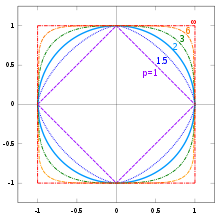
\includegraphics[width=0.6\textwidth]{assets/2.2 Norm/Lp-Norm in 2D space.png}
  \caption{$l_p$-norm in 2D space}
\end{figure}

Take $l_1$-norm as an example, its intersection points with the coordinate axis are sparse
because there are zeros. We call these points as \textbf{sparse points}. Imagine that there
is a funtion, there are countless points on the function, once intersecting with the sparse
points of $l_1$-norm, $l_1$-norm determines the sparse solution on the function. So that's
why $l_1$-norm proves sparsity.

\subsection{\textbf{Convex Optimization}}

\subsubsection{\textbf{Defination}}

For arbitrary $x, y$ and $\mu \in [0, 1]$, then $\mu x + (1-\mu)y$ means all points
on the line segment between $x$ and $y$. If $x, y$ are in a set $C$ and $\mu x + (1-\mu)y$
is also in $C$, then $C$ is called a \textbf{convex set}.

\begin{figure}[H]
  \centering
  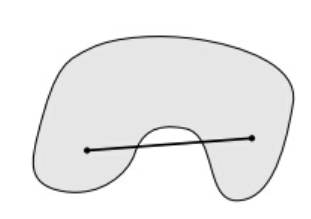
\includegraphics[width=0.4\textwidth]{assets/2.3 Convex Optimization/Not Convex Set.png}
  \caption{Not Convex Set}
\end{figure}

A function $f$ is called \textbf{convex function} if its domain is a convex set and for any
$x_1, x_2$ in the domain, the following inequality holds $f(\mu x_1 + (1-\mu)x_2) \leq \mu
 f(x_1) + (1-\mu)f(x_2)$.


If the inequality is strict, then $f$ is called a \textbf{strictly convex function}.

\begin{figure}[H]
  \centering
  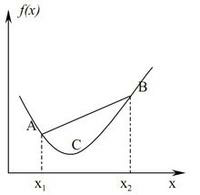
\includegraphics[width=0.4\textwidth]{assets/2.3 Convex Optimization/Convex Function.png}
  \caption{Convex Function}
\end{figure}

If we have such a optimization problem
\[
  \min_{x} f(x)
  \quad\text{s.t.}\quad
  g_i(x)\le 0,\;i=1,2,\dots,l,
\]
and$f(x), g_i(x)$ are all convex functions, then this is called a \textbf{convex
optimization problem}.

\subsubsection{\textbf{What's the usage?}}

If a problem can be represented as a convex optimization problem, then it can be solved
much easier. This is because we have many algorithms to solve convex optimization problems.

There are some non-convex optimization problems, but convex optimization can play a
significant role in solving them. For example, Lagrange Relaxation Algorithm's non-convex
condition can be converted to convex.

For convex optimization problems, local optimal solution is also the global optimal solution.
This is because the convex function has no local minimum, which means that the local minimum
is also the global minimum. This is a very important property of convex optimization.

\subsection{\textbf{Projection Matrix}}

\subsubsection{\textbf{Introdution}}

If you have learned Prof.Liu's Linear Algebra, you must have watched Prof. Gilbert Strang's
video about Linear Algebra. In this section we will talk about the projection matrix in
his 16th lecture.

If there are 3 points, (1, 1), (2, 2) and (3, 2), and we want to find a line to fit these
points, then we get a equation:
\[
  \begin{array}{c@{\;\;}c@{\;\;}c@{\;\;}c}
    \begin{bmatrix}1 & 1 \\ 1 & 2 \\ 1 & 3\end{bmatrix}
    & \begin{bmatrix}C \\ D\end{bmatrix}
    & = & \begin{bmatrix}1 \\ 2 \\ 2\end{bmatrix} \\\\
    A & x & = & b
  \end{array}
\]

It's clear that there is no solution to this equation, so we choose the least squares method
to find the best solution:
\[
  x = (A^TA)^{-1}A^Tb.
\]

And this introduces \textbf{projection matrix}.

\subsubsection{\textbf{Defination}}

Actually, solve x is a process that use the linear combination of the column vectors of $A$
to approximate $b$. We set a vector $p$ which is the most close to $b$ and is in the
column space of $A$. Then the question becomes $\min ||b-p||_2$. and $p$ is called the
\textbf{orthogonal projection} of $b$ onto the column space of $A$.

We set $\hat{x}$ is the solution of the least squares method, then we have:
\[
  p = A\hat{x} = A(A^TA)^{-1}A^Tb = Pb.
\]

The matrix $P = A(A^TA)^{-1}A^T$ is called the \textbf{projection matrix}.

\subsubsection{\textbf{Properties}}

Projection matrices have several important properties:

\begin{itemize}
  \item Symmetry: $P^T = P$.
  \item Idempotence: $P^2 = P$.
  \item Eigenvalues are only 0 or 1.
  \item For any vector $b$, $Pb$ is the orthogonal projection of $b$ onto $Col(A)$, and the residual $r = b - Pb$ satisfies $r \perp Col(A)$.
  \item If $A = Q R$ is a full QR factorization with $Q^T Q = I$, then $P = Q Q^T$.
\end{itemize}

\subsubsection{\textbf{Murmurs}}

When I was writing this section, I realized that I had forgotten most of the knowledge about
Linear Algebra. I had to quick review it before I wrote almost everything. Study is a
process of forgetting and remembering. So I suggest you to review the knowledge
regularly, not only the required courses but also things like this tutorial. Well, after this
subsection, we will go into the most important part, \textbf{Compressed Sensing}. Hope you
can understand it well.

\newpage
\thispagestyle{empty}
\begin{center}
    \vspace*{96pt}
    \fontsize{60}{60}\customfont{3}\par
    \fontsize{26}{31.2}\section{\textbf{Compressed Sensing}}\par % 标题
    \vspace{25pt}
    \fontsize{18}{21.6}\customfont{\textit{Ultimately you should follow advice not because
    someone tells you to, but because it was something that you already knew you should be
    doing. --- Terence Tao}}\par % 名言
    \vfill
\end{center}

\newpage
\subsection{\textbf{What is Compressed Sensing?}}

\subsubsection{\textbf{Theoretical Framework}}

Assume we have a $N$ long signal $X$, and $X$ can be sparsely represented by a orthogonal
basis $\Psi$, and we use a observation matrix $\Phi$ which is unrelated to $\Psi$, then We
get a observation signal $Y$, then reconstruct original signal $X$.

First, calculate the transformation factor $\Theta = \Psi^T$. Secondly, design a observation
matrix $\Phi$, then the observation signal $Y = \Psi \Theta = \Theta \Psi^T X$. Finally
this problem becomes a $l_0$-norm minimization problem:
\[
\min ||\Psi^T X||_0 \quad s.t. \quad Y = \Phi \Psi^T X.
\]

Compressed Sensing mainly includes 3 parts: signal's sparsity representation, observation
matrix design (also signal's low-speed sampling) and signal reconstruction.

\subsubsection{\textbf{Signal's Sparsity Representation}}

Under normal circumstances, we should choose specific basis $\Psi$, here is a table:

\begin{table}[H]
  \centering
  \begin{tabular}{|c|c|}
    \hline
    Application Scenario & Common Basis \\
    \hline
    1D signals      & Fourier basis, wavelets             \\
    Natural images  & DCT, wavelets, curvelets            \\
    ECG signals     & Wavelets                            \\
    Audio signals   & Gabor frames, Fourier basis         \\
    Video signals   & 3D DCT, wavelets                    \\
    MRI images      & Wavelets, curvelets                 \\
    \hline
  \end{tabular}
  \caption*{Common bases for different application scenarios}
\end{table}

\subsubsection{\textbf{Observation Matrix Design}}

The core property of the observation matrix $\Phi$ is \textbf{Restrict Isometry (RIP)}.
RIP means that $\Phi$ can preserve the distance between the sparse signal and its
observation. In other words, $\Phi$ can ensure that the sparse signal can be reconstructed
from its observation. However, the RIP is very hard to satisfy, and there's a equivalent
conditions$^{[4]}$ for RIP: \textbf{Incorrectness between the observation matrix $\Phi$ and
the basis $\Psi$}. For most cases, \textbf{random Gaussian matrix} can satisfy this
condition. There are also some other matrices, we will show them soon.

Here's a figure to show Compressed Sensing$^{[5]}$, the observation matrix $\Phi$ is a
random Gaussian matrix, the basis $\Psi$ is a DCT basis.

\begin{figure}[H]
  \centering
  \includegraphics[width=0.95\textwidth]{assets/3.1 What is Compressed Sensing/Compressed
  Sensing.png}
  \caption{Compressed Sensing}
\end{figure}

\subsubsection{\textbf{Signal Reconstruction}}

We have talked that Compressed Sensing can be transformed to a $l_1$-norm minimization
problem, and this is a convex optimization problem ($l_1$-norm is convex and the equation
is also convex). There are 3 kinds of methods to solve this problem: \textbf{Convex Relaxation
Method}, \textbf{Greedy Pursuit Method} and \textbf{Iterative Thresholding Method}.

The typical representative of convex relaxation method is \textbf{Basic Pursuit (BP)},
\textbf{Basic Pursuit Denoising (BPDN)}, while greedy pursuit method is \textbf{Orthogonal
Matching Pursuit (OMP)} and \textbf{Compressive Sampling Matching Pursuit (CoSaMP)}. 
Iterative thresholding method is \textbf{Iterative Hard Thresholding (IHT)} and
\textbf{Iterative Soft Thresholding (IST)}. Every Algorithm has its own advantages and
disadvantages, and the choice of algorithm depends on the specific application scenario.
We will discuss greedy pursuit method in this tutorial.

\subsection{\textbf{Common Observation Matrices}}

\subsubsection{\textbf{Random Gaussian Matrix}}

Random Guassian Matrix is the most commonly used observation matrix in Compressed Sensing.
Make a $M \times N$ matrix $\Phi$, and every elements obey Gaussian distribution
$N (0,\frac{1}{M})$. That is to say:
\[
  \Phi_{ij} \sim N(0, \frac{1}{M}).
\]

This matrix has a high probability of meeting the RIP condition, and need not very large
measurements.

Here's a simple example in MATLAB:

\begin{lstlisting}[language=Matlab]
%% Random Gaussian Matrix Example
Phi = randn(M, N) / sqrt(M);
\end{lstlisting}

\subsubsection{\textbf{Random Bernoulli Matrix}}

Random Bernoulli Matrix is a special case of random Gaussian matrix. It is a $M \times N$
matrix, and every elements obey Bernoulli distribution:
\[
  \Phi_{ij} = \frac{1}{\sqrt{M}}
  \begin{cases}
    +1 \quad P=\tfrac12 \\
    -1 \quad P=\tfrac12
  \end{cases}
  \text{or} \quad
  \Phi_{ij} = \frac{3}{\sqrt{M}}
  \begin{cases}
    +1 \quad P=\tfrac16 \\
    0 \quad P=\tfrac23 \\
    -1 \quad P=\tfrac16
  \end{cases}
\]

This matrix is more convient to storage and transmission than random Gaussian matrix.

Here's a simple example in MATLAB:

\begin{lstlisting}[language=Matlab]
%% Random Bernoulli Matrix Example
Phi = randi([0, 1], M, N)
Phi(Phi == 0) = -1;
Phi = Phi / sqrt(M);
\end{lstlisting}

\subsubsection{\textbf{Sparse Random Measurement Matrix}}

Make a all-zero $M \times N (M < N)$ matrix $\Phi$, randomly choose $d (d < M)$ positions in each
columns and set them to 1. There isn't much difference when $d = \{4, 8, 10, 16\}$. This matrix
is also easy to storage.

Here's a simple example in MATLAB:

\begin{lstlisting}[language=Matlab]
%% Sparse Random Measurement Matrix Example
Phi = zeros(M, N);
for i = 1:N
    idx = randperm(M, d);
    Phi(idx, i) = 1;
end
\end{lstlisting}

\subsubsection{\textbf{Toeplitz Matrix}}

We define a Toeplitz matrix as:
\[
  T = \begin{bmatrix}
    t_n & t_{n-1} & \cdots & t_1 \\
    t_{n+1} & t_n & \cdots & t_2 \\
    \vdots & \vdots & \ddots & \vdots \\
    t_{2n-1} & t_{2n-2} & \cdots & t_n
  \end{bmatrix}
\]

When we construct a Toeplitz matrix, set a random vector $u = (u_1, u_2, \ldots, u_n)$ and
do a $M (M < N)$ times loop to construct $M-1$ rows. Then normalize the matrix at last.
Usually the value of $u$ is $\pm 1$ and obey Bernoulli distribution like random Bernoulli
matrix. In practice, the application prospects of T-matrix are relatively good because
cyclic displacement is easy to implement in hardware.

Here's a simple example in MATLAB:

\begin{lstlisting}[language=Matlab]
%% Toeplitz Matrix Example
u = randi([0, 1], 1, 2*N-1);
u(u == 0) = -1;

Phi = toeplitz(u(N:end), fliplr(u(1:N)));
Phi = Phi(1:M, :);
\end{lstlisting}

\subsection{\textbf{Greedy Pursuit Method}}

\subsubsection{\textbf{Introduction}}

When $A$ and $x$ are known, it's easy to solve $y = Ax$. But if $A$ and $y$ is known,
how to calculate $x$?

A way is that $x = A^{-1}y$, but we know the inverse matrix is hard to calculate,
and the matrix $A$ may not be invertible. So we need a new way to solve this problem.
This is the original idea of Matching Pursuit (MP).

However, MP has many problems, to solve these problems, a very important algorithm
called \textbf{Orthogonal Matching Pursuit (OMP)} was proposed. OMP is a typical greedy
pursuit algorithm, In this section, we will introduce OMP and its variants.

\subsubsection[\textbf{Examples}]{\textbf{Examples}\textsuperscript{[6]}}

\paragraph{\textbf{Example 1}}\mbox{}\\
\[
  y = \begin{bmatrix} 1.65 \\ -0.25 \end{bmatrix}, \quad
  A = \begin{bmatrix} -0.707 & 0.8 & 0 \\ 0.707 & 0.6 & -1 \end{bmatrix}
\]

$A$ can be represented as a set of column vectors, and these vectors are called
\textbf{atoms}. The goal of OMP is to find a linear combination of these atoms to
reconstruct $y$. So we need to find which atom contributes to $y$ most, and which
second, and so on. This process iterates N times, where N is the number of atoms.
In this example, N = 3.

Contribution $\omega_i$ is $|<b_i, y>|$ or $|b_i^Ty|$. In this example, we have:
\[
  \omega = \begin{bmatrix}
    |<b_1, y>| \\
    |<b_2, y>| \\
    |<b_3, y>|
  \end{bmatrix}
  = \begin{bmatrix}
    |-1.34| \\
    |1.17| \\
    |0.25|
  \end{bmatrix}
\]

So we choose $b_1$ as the first atom, write it into a new matrix $A_{new}$, then
calculate residual $r = y - b_1\omega_1 = \begin{bmatrix} 0.7 \\ 0.7 \end{bmatrix}$.
Also, create a contribution matrix $x_{rec} = \begin{bmatrix} -1.34 \\ 0 \\ 0
\end{bmatrix}$ to record the contribution of $A_{new}$ to $y$ \textbf{(Not $\omega$!)}.

Actually, every time we calculate $x_{rec}$, least squares method is needed.
Because $b_i$ is normalized ($l_1$-norm is 1) in this example, we can use $w_i$ for
the first time. We will talk about this later.

Then we repeat this process, calculate the contribution of $b_2$ and $b_3$ to $r$,
and choose $b_2$ as the second atom, write it into $A_{new}$, and calculate $x_{rec}$.

To calculate $x_{rec}$, we need to calculate $\lambda$ that makes $\sum \lambda_i b_i$
most close to $y$. This is a least squares problem, like following equation:
\[
  \min ||A_{new} \cdot \lambda - y||_2
\]

The solution is:
\[
  \lambda = (A_{new}^TA_{new})^{-1}A_{new}^Ty.
\]

And sometimes QR decomposition is used to solve this equation, which is more stable.
\[
  A_{new} = QR \Rightarrow \lambda = R^{-1}Q^Ty.
\]

Upon completing this, we have $x_{rec} = \begin{bmatrix} -1.2 \\ 1 \\ 0 \end{bmatrix}$,
now $r = y - A_{new} \cdot \lambda = \begin{bmatrix} 0 \\ 0 \end{bmatrix}$.  This is the
answer.

\paragraph{\textbf{Example 2}}\mbox{}\\
\[
  y = \begin{bmatrix} 2.7 \\ 0.1 \\ 4.5\end{bmatrix}, \quad 
  A = \begin{bmatrix} -0.8 & 0.3 & 1 & 0.4 \\ -0.2 & 0.4 & -0.3 & -0.4 \\
  0.2 & 1 & -0.1 & 0.8 \end{bmatrix}
\]

Normalize the atoms:
\[
  \hat{b_1} = \begin{bmatrix}-0.9428 \\ -0.2357 \\ 0.2357\end{bmatrix}, \quad
  \hat{b_2} = \begin{bmatrix}0.2680 \\ 0.3578 \\ 0.8940\end{bmatrix}, \quad
  \hat{b_3} = \begin{bmatrix}0.9535 \\ -0.2860 \\ 0.0953\end{bmatrix}, \quad
  \hat{b_4} = \begin{bmatrix}0.4082 \\ -0.4082 \\ -0.8165\end{bmatrix}
\]

Calculate $\omega$:
\[
  \omega = \hat{A}^Ty = \begin{bmatrix} -1.5085 \\ 4.7852 \\ 2.1167 \\ 4.7357
  \end{bmatrix}
\]

Add $b_2$ to $A_{new}$, calculate $x_{rec}$:
\[
  L_p = (A_{new}^TA_{new})^{-1}A_{new}^Ty = \begin{bmatrix} 4.28 \end{bmatrix} \quad
  x_{rec} = \begin{bmatrix} 0 \\ 4.28 \\ 0 \\ 0 \end{bmatrix}
\]

Then residual:
\[
  r = y - A_{new} \cdot L_p = \begin{bmatrix} 1.416 \\ -1.612 \\ 0.22 \end{bmatrix}
\]

Repeat this process, we get the final result:
\[
  x_{rec} = \begin{bmatrix} 0 \\ 3 \\ 1 \\ 2 \end{bmatrix}
\]

\subsubsection{\textbf{Summrize}}

Sometimes the sparsity level $K$ is known, which means we know how many atoms we need
to choose. In this case, we can stop after $K$ iterations.

The steps of OMP are:
\begin{enumerate}
  \item Normalize the atoms.
  \item Calculate the contribution $\omega$ of each atom.
  \item Choose the atom with the largest contribution and add it to $A_{new}$.
  \item Calculate $x_{rec}$ using least squares method.
  \item Update the residual $r = y - A_{new} \cdot x_{rec}$.
  \item Repeat steps 2-5 until the number of iterations reaches $K$ or all atoms are
  used or the residual is small enough.
\end{enumerate}

In the fact, OMP's calculation step is to normalize each atom by \textbf{Gram-Schmidt
Orthogonalization}, then subtract the orthogonalized components from the signal to be
decomposed to obtain the residual. More about Gram-Schmidt Orthogonalization
can be found in Prof.Strang's Linear Algebra course.

\subsubsection{\textbf{Variants}}

\paragraph{\textbf{Compressive Sampling Matching Pursuit (CoSaMP)}}\mbox{}\\
OMP choose 1 atom which has the largest contribution each time, but CoSaMP choose
$2K$ atoms, then cut the support set $A$ to $K$ atoms. This makes CoSaMP more
efficient than OMP, especially when the number of atoms is large (or longer
signal with noisy).

\paragraph{\textbf{Subspace Pursuit (SP)}}\mbox{}\\
SP is a variant of CoSaMP, it chooses $K$ atoms each time. Its accuracy and complexity
are between CoSaMP and BP (however, I can't produce a high accuracy result with BP no
matter what toolbox I tried, that's wierd).

\paragraph{\textbf{Sparsity Adaptive Matching Pursuit (SAMP)}}\mbox{}\\
SAMP is distinguished from OMP and CoSaMP because it is sparsity adaptived. It
uses a step $S$ to adaptive the sparsity level. At the first time, let $L = S$,
choose $L$ atoms, and cut the support set to $L$ atom each iterations. If the
residual stops decreasing, then let $L = L + S$. Fianally $L \approx K$.

\subsubsection{\textbf{MATLAB Example}}

\paragraph{\textbf{OMP}}
\begin{lstlisting}[language=Matlab]
%% OMP_example
clear; clc; close all;
rng(42);

%% Parameters
N = 500;               % signal length
Fs = 1000;             % sampling frequency
T = N/Fs;              % signal duration
t = (0:N-1)/Fs;        % time vector

sparsity_level = 8;    % estimated sparsity
loss_percentage = 0.3; % 30% data loss
noise_level = 0.1;     % noise level

%% Signal Generation
% frequency components
freqs = [10, 25, 40, 60];
amps = [1.0, 0.8, 0.6, 0.4];

x_original = zeros(1, N);
for i = 1:length(freqs)
    x_original = x_original + amps(i) * sin(2*pi*freqs(i)*t);
    if mod(i, 2) == 0
        x_original = x_original + 0.7*amps(i) * cos(2*pi*freqs(i)*t);
    end
end

% normalization
x_original = x_original / max(abs(x_original));
x_original = x_original(:);

%% Data Loss and Noise
mask = rand(N, 1) > loss_percentage;
x_observed = x_original .* mask + noise_level*randn(N,1);

%% Construct Observation System
obs_idx = find(mask);
M       = length(obs_idx);
y       = x_observed(obs_idx);
A = zeros(M, N);
for i = 1:M
    A(i, obs_idx(i)) = 1;
end

%% Construct DCT Sparse Basis and Sensing Matrix
Psi = dctmtx(N)';
% normalize basis vectors
for i = 1:N
    Psi(:, i) = Psi(:, i) / norm(Psi(:, i));
end

% sensing matrix
Phi = A * Psi;
% normalize columns
col_norms = sqrt(sum(Phi.^2, 1));
col_norms(col_norms < eps) = 1;
Phi = Phi ./ col_norms;

%% OMP
max_iter = 33;          % maximum iterations
residual = y;           % initial residual
index_set = [];         % support set
theta_hat = zeros(size(Psi, 2), 1);  % sparse coefficients estimate
res_history = zeros(max_iter, 1);    % residual history
selected_atoms = false(size(Psi, 2), 1); % track selected atoms

% OMP main loop
for iter = 1:max_iter
    % compute projections of residual onto sensing matrix
    projections = abs(Phi' * residual);
    projections(selected_atoms) = -inf; % exclude selected atoms
    % find index of max projection
    [max_val, new_idx] = max(projections);
    % check if atom found
    if max_val < 1e-6 || isinf(max_val)
        break;
    end
    % mark and add new atom
    selected_atoms(new_idx) = true;
    index_set = [index_set, new_idx];
    % build submatrix with selected atoms
    Phi_sub = Phi(:, selected_atoms);
    % least squares solution
    if iter == 1
        Q = Phi_sub / norm(Phi_sub);
        R = 1;
        x_ls = Q' * y;
    else
        [Q, R] = qr(Phi_sub, 0);
        x_ls = R \ (Q' * y);
    end
    % update residual
    residual = y - Phi_sub * x_ls;
    res_history(iter) = norm(residual);
    % check stopping criteria
    if norm(residual) < 1e-4 || iter >= max_iter
        break;
    end
end

% build sparse coefficient estimate
theta_hat(selected_atoms) = x_ls;

%% Reconstruct Signal
x_reconstructed = Psi * theta_hat;
x_final = x_reconstructed;
x_final(obs_idx) = x_observed(obs_idx);

%% Result Visualization
figure('Position', [100, 100, 900, 800], 'Name', 'OMP Reconstruction Results');

% Time domain
subplot(4,1,1);
plot(t, x_original, 'b', 'LineWidth', 1.8);
hold on;
stem(t, x_observed, 'r', 'Marker', 'o', 'MarkerSize', 3, 'MarkerFaceColor', 'r');
title(['Original and Observed Signals (Data loss: ', num2str(loss_percentage*100), '%, Noise level: ', num2str(noise_level), ')']);
legend('Original signal', 'Observed samples', 'Location', 'best');
xlabel('Time');
ylabel('Amplitude');
xlim([0, T]);
grid on;

subplot(4,1,2);
plot(t, x_original, 'b', 'LineWidth', 1.8);
hold on;
plot(t, x_final, 'r--', 'LineWidth', 1.5);
title('Original vs Reconstructed (Time domain)');
legend('Original signal', 'OMP', 'Location', 'best');
xlabel('Time');
ylabel('Amplitude');
xlim([0, T]);
grid on;

% Reconstruction error
subplot(4,1,3);
error_signal = x_original - x_final;
plot(t, error_signal, 'g', 'LineWidth', 1.5);
title('Reconstruction Error');
xlabel('Time');
ylabel('Error');
xlim([0, T]);
grid on;

% Frequency domain
subplot(4,1,4);
freq = linspace(0, Fs/2, floor(N/2)+1);
Y_orig = fft(x_original);
P_orig = abs(Y_orig(1:floor(N/2)+1)/N);
Y_rec = fft(x_final);
P_rec = abs(Y_rec(1:floor(N/2)+1)/N);

plot(freq, 20*log10(P_orig), 'b', 'LineWidth', 1.5);
hold on;
plot(freq, 20*log10(P_rec), 'r--', 'LineWidth', 1.2);
title('Original vs Reconstructed (Frequency domain)');
xlabel('Frequency');
ylabel('Magnitude (dB)');
legend('Original signal', 'Reconstructed', 'Location', 'best');
xlim([0, 100]);
grid on;

%% Compute Reconstruction Metrics
% final error
error_final = x_original - x_final;
rel_error_final = norm(error_final) / norm(x_original);

fprintf('===== Reconstruction Result Statistics =====\n');
fprintf('Signal length: %d\n', N);
fprintf('Sampling frequency: %d Hz\n', Fs);
fprintf('Data loss percentage: %.1f%%\n', loss_percentage*100);
fprintf('Number of observations: %d (%.1f%%)\n', M, (M/N)*100);
fprintf('Sparse basis: DCT\n');
fprintf('Estimated sparsity: %d\n', sparsity_level);
fprintf('OMP iterations: %d\n', iter);
fprintf('Relative reconstruction error: %.4f\n', rel_error_final);
\end{lstlisting}

Here's the result of the MATLAB example:

\begin{verbatim}
===== Reconstruction Result Statistics =====
Signal length: 500
Sampling frequency: 1000 Hz
Data loss percentage: 30.0%
Number of observations: 346 (69.2%)
Sparse basis: DCT
Estimated sparsity: 8
OMP iterations: 33
Relative reconstruction error: 0.2097
\end{verbatim}

\begin{figure}[H]
  \centering
  \includegraphics[width=0.8\textwidth]{assets/3.3 Greedy Pursuit Method/MATLAB OMP
  Example.png}
  \caption{MATLAB OMP Example}
\end{figure}

\newpage
\paragraph{\textbf{CoSaMP}}
\begin{lstlisting}[language=Matlab]
%% CoSaMP_example
clear; clc; close all;
rng(42);

%% Parameters
N = 4000;              % signal length
Fs = 1000;             % sampling frequency
T = N/Fs;              % signal duration
t = (0:N-1)/Fs;        % time vector

sparsity_level = 8;    % target sparsity
loss_percentage = 0.97;% data loss ratio
noise_level = 0.1;     % noise level

%% Signal Generation
freqs = [10, 25, 40, 60];
amps  = [1.0, 0.8, 0.6, 0.4];
x_original = zeros(1, N);
for i = 1:length(freqs)
    x_original = x_original + amps(i)*sin(2*pi*freqs(i)*t);
    if mod(i,2)==0
        x_original = x_original + 0.7*amps(i)*cos(2*pi*freqs(i)*t);
    end
end
x_original = x_original / max(abs(x_original));
x_original = x_original(:);

%% Data Loss and Noise
mask       = rand(N,1) > loss_percentage;
x_observed = x_original .* mask + noise_level*randn(N,1);

%% Construct Observation System
obs_idx = find(mask);
M       = length(obs_idx);
y       = x_observed(obs_idx);
A = zeros(M, N);
for i = 1:M
    A(i, obs_idx(i)) = 1;
end

%% Construct DFT Sparse Basis and Sensing Matrix
Psi = dftmtx(N) / sqrt(N);
for i = 1:N
    Psi(:,i) = Psi(:,i) / norm(Psi(:,i));
end
Phi = A * Psi;

%% CoSaMP
max_iter    = 10;
K           = sparsity_level;
residual    = y;
theta_hat   = zeros(N,1);
support_set = [];
res_history = zeros(max_iter,1);

for iter = 1:max_iter
    % 1. Residual correlations
    correlations = abs(Phi' * residual);
    % 2. Select 2K atoms
    [~, idx]      = sort(correlations,'descend');
    candidate_set = idx(1:min(2*K, length(idx)));
    % 3. Merge support set
    merged_set    = union(support_set, candidate_set);
    % 4. Least squares estimation
    Phi_sub = Phi(:, merged_set);
    x_ls    = Phi_sub \ y;
    % 5. Keep K largest coefficients
    [~, sidx]   = sort(abs(x_ls),'descend');
    support_set = merged_set(sidx(1:min(K, length(x_ls))));
    % 6. Update sparse coefficients
    theta_hat(support_set) = Phi(:, support_set) \ y;
    % 7. Update residual
    residual = y - Phi(:, support_set) * theta_hat(support_set);
    res_history(iter) = norm(residual);
    if res_history(iter) < 1e-6
        break;
    end
end

%% Reconstruct Signal
x_reconstructed = Psi * theta_hat;
x_final         = real(x_reconstructed);
x_final = medfilt1(x_final, 7);

%% Result Visualization
figure('Position',[100,100,900,800],'Name','CoSaMP Reconstruction Results');

% Time domain
subplot(4,1,1);
plot(t, x_original,'b','LineWidth',1.8); hold on;
stem(t, x_observed, 'r','Marker','o','MarkerSize',3,'MarkerFaceColor','r');
title(['Original Signal and Observations (Data loss: ',num2str(loss_percentage*100),'%, Noise level: ',num2str(noise_level),')']);
legend('Original signal','Observed samples'); xlabel('Time'); ylabel('Amplitude');
xlim([0,T]); grid on;

subplot(4,1,2);
plot(t, x_original,'b','LineWidth',1.8); hold on;
plot(t, x_final,'r--','LineWidth',1.5);
title('Original vs Reconstructed (Time domain)');
legend('Original signal','CoSaMP'); xlabel('Time'); ylabel('Amplitude');
xlim([0,T]); grid on;

% Reconstruction error
subplot(4,1,3);
error_signal = x_original - x_final;
plot(t, error_signal,'g','LineWidth',1.5);
title('Reconstruction Error'); xlabel('Time'); ylabel('Error');
xlim([0,T]); grid on;

% Frequency domain
subplot(4,1,4);
halfN = floor(N/2) + 1;
freq  = linspace(0, Fs/2, halfN);
Y_o   = fft(x_original);
P_o   = abs(Y_o(1:halfN)/N);
P_o(2:end-1) = 2*P_o(2:end-1);
Y_r   = fft(x_final);
P_r   = abs(Y_r(1:halfN)/N);
P_r(2:end-1) = 2*P_r(2:end-1);
P_o_db = 20*log10(P_o + eps);
P_r_db = 20*log10(P_r + eps);
plot(freq, P_o_db,'b','LineWidth',1.5); hold on;
plot(freq, P_r_db,'r--','LineWidth',1.2);
title('Original vs Reconstructed (Frequency domain)');
xlabel('Frequency (Hz)'); ylabel('Magnitude (dB)');
legend('Original signal','Reconstructed'); xlim([0,100]); grid on;
ylim([-50, 0]);

%% Performance Metrics
error_final     = x_original - x_final;
rel_error_final = norm(error_final)/norm(x_original);

fprintf('===== CoSaMP Reconstruction Result Statistics =====\n');
fprintf('Signal length: %d\n', N);
fprintf('Sampling frequency: %d Hz\n', Fs);
fprintf('Data loss percentage: %.1f%%\n', loss_percentage*100);
fprintf('Number of observations: %d (%.1f%%)\n', M, (M/N)*100);
fprintf('Sparse basis: DFT\n');
fprintf('Target sparsity: %d\n', sparsity_level);
fprintf('CoSaMP iterations: %d\n', iter);
fprintf('Relative reconstruction error: %.4f\n', rel_error_final);
\end{lstlisting}

Here's the result of the MATLAB example:

\begin{verbatim}
===== CoSaMP Reconstruction Result Statistics =====
Signal length: 4000
Sampling frequency: 1000 Hz
Data loss percentage: 97.0%
Number of observations: 111 (2.8%)
Sparse basis: DFT
Target sparsity: 8
CoSaMP iterations: 10
Relative reconstruction error: 0.1074
\end{verbatim}

\begin{figure}[H]
  \centering
  \includegraphics[width=0.8\textwidth]{assets/3.3 Greedy Pursuit Method/MATLAB CoSaMP
  Example.png}
  \caption{MATLAB CoSaMP Example}
\end{figure}

That's crazy that CoSaMP can reconstruct the signal with only 2.8\% observations and
90\% precision. 

\paragraph{\textbf{SAMP}}
\begin{lstlisting}[language=Matlab]
%% SAMP_example
clear; clc; close all;
rng(42);

%% Parameters
N = 4000;              % signal length
Fs = 1000;             % sampling frequency
T = N/Fs;              % signal duration
t = (0:N-1)/Fs;        % time vector

loss_percentage = 0.97;% data loss ratio
noise_level = 0.1;     % noise level

%% Signal Generation
freqs = [10, 25, 40, 60];
amps  = [1.0, 0.8, 0.6, 0.4];
x_original = zeros(1, N);
for i = 1:length(freqs)
    x_original = x_original + amps(i)*sin(2*pi*freqs(i)*t);
    if mod(i,2)==0
        x_original = x_original + 0.7*amps(i)*cos(2*pi*freqs(i)*t);
    end
end
x_original = x_original / max(abs(x_original));
x_original = x_original(:);

%% Data Loss and Noise
mask       = rand(N,1) > loss_percentage;
x_observed = x_original .* mask + noise_level*randn(N,1);

%% Construct Observation System
obs_idx = find(mask);
M       = length(obs_idx);
y       = x_observed(obs_idx);
A = zeros(M, N);
for i = 1:M
    A(i, obs_idx(i)) = 1;
end

%% Construct DFT Sparse Basis and Sensing Matrix
Psi = dftmtx(N) / sqrt(N);
for i = 1:N
    Psi(:,i) = Psi(:,i) / norm(Psi(:,i));
end
Phi = A * Psi;

%% SAMP Algorithm Parameters
step_size       = 2;          % step size
max_sparsity    = 20;         % maximum allowed sparsity
max_iter        = 50;         % maximum iterations
residual        = y;          % initial residual
theta_hat       = zeros(N,1); % sparse coefficient estimate
support_set     = [];         % support set
L               = step_size;  % current stage sparsity estimate
prev_res_norm   = inf;        % previous residual norm
res_history     = [];         % residual history

%% SAMP
iter = 0;
stage = 1;
converged = false;

while ~converged && iter < max_iter && L <= max_sparsity
    iter = iter + 1;
    % 1. Compute residual correlations
    correlations = abs(Phi' * residual);
    % 2. Select L most correlated atoms
    [~, idx] = sort(correlations, 'descend');
    candidate_set = idx(1:min(L, length(idx)));
    % 3. Merge support set
    merged_set = union(support_set, candidate_set);
    % 4. Least squares estimation
    Phi_sub = Phi(:, merged_set);
    x_ls = pinv(Phi_sub) * y;  % use pseudo-inverse for stability
    % 5. Keep L largest coefficients
    [~, sidx] = sort(abs(x_ls), 'descend');
    selected_indices = sidx(1:min(L, length(x_ls)));
    support_set_new = merged_set(selected_indices);
    % 6. Update coefficients on support set
    Phi_sub_new = Phi(:, support_set_new);
    theta_ls = pinv(Phi_sub_new) * y;
    % 7. Compute new residual
    residual_new = y - Phi_sub_new * theta_ls;
    res_norm = norm(residual_new);
    res_history(iter) = res_norm;
    % 8. Residual comparison
    if res_norm < prev_res_norm
        % residual decreased: accept update and stay in this stage
        support_set = support_set_new;
        residual = residual_new;
        theta_hat = zeros(N,1);
        theta_hat(support_set) = theta_ls;
        prev_res_norm = res_norm;
        % check convergence
        if res_norm < 1e-6
            converged = true;
            fprintf('SAMP converged at stage %d (L=%d)\n', stage, L);
        end
    else
        % residual did not decrease: move to next stage
        L = L + step_size;
        stage = stage + 1;
        prev_res_norm = inf;  % reset residual benchmark
    end
end

%% Reconstruct Signal
x_reconstructed = Psi * theta_hat;
x_final = real(x_reconstructed);
x_final = medfilt1(x_final, 7);

%% Result Visualization
figure('Position',[100,100,900,800],'Name','SAMP Reconstruction Results');

% Time domain
subplot(4,1,1);
plot(t, x_original,'b','LineWidth',1.8); hold on;
stem(t, x_observed, 'r','Marker','o','MarkerSize',3,'MarkerFaceColor','r');
title(['Original Signal and Observations (Data loss: ',num2str(loss_percentage*100),'%, Noise level: ',num2str(noise_level),')']);
legend('Original','Observed samples'); xlabel('Time'); ylabel('Amplitude');
xlim([0,T]); grid on;

subplot(4,1,2);
plot(t, x_original,'b','LineWidth',1.8); hold on;
plot(t, x_final,'r--','LineWidth',1.5);
title('Original vs Reconstructed (Time domain)');
legend('Original','SAMP'); xlabel('Time'); ylabel('Amplitude');
xlim([0,T]); grid on;

% Reconstruction error
subplot(4,1,3);
error_signal = x_original - x_final;
plot(t, error_signal,'g','LineWidth',1.5);
title('Reconstruction Error'); xlabel('Time'); ylabel('Error');
xlim([0,T]); grid on;

% Frequency domain
subplot(4,1,4);
halfN = floor(N/2) + 1;
freq  = linspace(0, Fs/2, halfN);
Y_o   = fft(x_original);
P_o   = abs(Y_o(1:halfN)/N);
P_o(2:end-1) = 2*P_o(2:end-1);
Y_r   = fft(x_final);
P_r   = abs(Y_r(1:halfN)/N);
P_r(2:end-1) = 2*P_r(2:end-1);
P_o_db = 20*log10(P_o + eps);
P_r_db = 20*log10(P_r + eps);
plot(freq, P_o_db,'b','LineWidth',1.5); hold on;
plot(freq, P_r_db,'r--','LineWidth',1.2);
title('Original vs Reconstructed (Frequency domain)');
xlabel('Frequency (Hz)'); ylabel('Magnitude (dB)');
legend('Original','Reconstructed'); xlim([0,100]); grid on;
ylim([-50, 0]);

%% Performance Metrics
error_final = x_original - x_final;
rel_error_final = norm(error_final)/norm(x_original);

fprintf('===== SAMP Reconstruction Result Statistics =====\n');
fprintf('Signal length: %d\n', N);
fprintf('Sampling frequency: %d Hz\n', Fs);
fprintf('Data loss percentage: %.1f%%\n', loss_percentage*100);
fprintf('Number of observations: %d (%.1f%%)\n', M, (M/N)*100);
fprintf('Sparse basis: DFT\n');
fprintf('Step size: %d\n', step_size);
fprintf('Final sparsity estimate: %d\n', L);
fprintf('Total iterations: %d\n', iter);
fprintf('Relative reconstruction error: %.4f\n', rel_error_final);
\end{lstlisting}

Here's the result of the MATLAB example:

\begin{verbatim}
===== SAMP Reconstruction Result Statistics =====
Signal length: 4000
Sampling frequency: 1000 Hz
Data loss percentage: 97.0%
Number of observations: 111 (2.8%)
Sparse basis: DFT
Step size: 2
Final sparsity estimate: 22
Total iterations: 22
Relative reconstruction error: 0.1082
\end{verbatim}

\begin{figure}[H]
  \centering
  \includegraphics[width=0.8\textwidth]{assets/3.3 Greedy Pursuit Method/MATLAB SAMP
  Example.png}
  \caption{MATLAB SAMP Example}
\end{figure}

Some of my opinion, SAMP is the best greedy pursuit algorithm in practice because it
is accurate as CoSaMP and don't have to give the sparsity level $K$ in advance. This
is a critical point for engineering applications, because we don't know how many
atoms we need to choose in most cases.

\section*{\textbf{Afterword}}
\addcontentsline{toc}{section}{Afterword}

This tutorial is hastily ended here. Some may ask why I didn't introduce more
algorithms like BP or IHT or something, you may think that I am lazy or I even don't
learn them. However, I had tried them but unfortunately I can't get a good result with
them. All papers I read said convex optimization method gets the best result, but I just
have no chance. Hmm,  maybe I mistakes something, or I didn't try hard enough.

I know, i know. Learning can't be always successful, and I had met many failures
in writing this tutorial. But I still finished it, though a rough version. I hope
this tutorial can help you to learn the ABC of Compressed Sensing, and in certain ways,
to help you to learn the ABC of studying.

After this tutorial, I will continue to work on my project. You know, I will go into
my third year of college, and I must start to think about lots of things, like
graduate recommendation, awards, and even my future. If you are my junior, I hope
you can learn to think, and study for yourself. This is also what I talked in the
last Linux tutorial. Don't always regret it until it's end.

Well, the next tutorial may be Linear Algebra. That's because Teacher Chen told me
that starting from the 2025th EE major, Linear Algebra will be taught by the College
of Science, not Prof. Liu. I feel bad about this. So I think I need a tutorial to
generalize Prof. Strang's Linear Algebra course, which can be a reference for
EE students in the future. I will try to finish it before the mid of 2026.

So let's end here. Class is over, dimiss!

\begin{flushright}
  Lancet Ross\\
  Jul 30th, 2025
\end{flushright}

\newpage
\section*{\textbf{References}}
\addcontentsline{toc}{section}{References}
\begin{enumerate}[label={[\arabic*]}, leftmargin=0pt]
  \raggedright
  \item POLIKAR R. The Wavelet Tutorial [EB/OL]. Rowan University, (2006) [2025-07-19].
  \url{https://users.rowan.edu/~polikar/WTtutorial.html}.
  \item Bala Priya C. L1 Norm Regularization and Sparsity Explained for Dummies[EB/OL].
  ML Review, 2016-08-27 [2025-07-20]. \url{https://blog.mlreview.com/l1-norm-
  regularization-and-sparsity-explained-for-dummies-5b0e4be3938a}.
  \item 半度墨水. 什么是范数[EB/OL]. 博客园, 2023-05-26 [2025-07-20] \url{https://www.cnblogs.
  com/HOI-Yzy/p/17435192.html}.
  \item R Baraniuk. A lecture on compressive sensing[J]. IEEE Signal Processing Magazine,
  2007, 24(4): 118-121.
  \item 石光明,刘丹华,高大化,等.压缩感知理论及其研究进展[J].电子学报,2009,37(05):1070-1081.
  \item Koredianto Usman. Introduction to Orthogonal Matching Pursuit[EB/OL].
  2017-08-30 [2025-07-20] \url{https://korediantousman.staff.telkomuniversity.ac.id/
  files/2017/08/main-1.pdf}
\end{enumerate}

\end{document}